\documentclass[coursework, och]{SCWorks1}

\usepackage[utf8]{inputenc}
\usepackage{cmap}
\usepackage[T2A]{fontenc}

\usepackage{graphicx}
\usepackage{float}

\usepackage[sort,compress]{cite}
\usepackage{amsmath}
\usepackage{amssymb}
\usepackage{amsthm}
\usepackage{fancyvrb}
\usepackage{longtable}
\usepackage{array}
\usepackage[english,russian]{babel}

\usepackage[colorlinks=false]{hyperref}

\renewcommand{\labelenumii}{\arabic{enumi}.\arabic{enumii}.}

\newcommand{\eqdef}{\stackrel {\rm def}{=}}

\newtheorem{lem}{Лемма}
\newtheorem{definition}{Определение}

\begin{document}


%=================================================================================
\textbf{1 Метод Гаусса решения СЛАУ}

Задача: решить СЛАУ $Ax = b$ методом Гаусса с выбором главного элемента в столбце, где
\[
A = \begin{pmatrix}
    3 & 1 & -1 & 0 & 3 & 2 \\
    1 & -2 & 0.5 & 4 & -1 & 3 \\
    0 & 3 & 1 & -2 & 2 & 1 \\
    1 & 0 & -3 & 2 & 1 & -1 \\
    2 & -1 & 1 & 3 & -2 & 0.5 \\
    -1 & 2 & 0 & 1 & 4 & -3
\end{pmatrix}
\quad
b = \begin{pmatrix}
    4 \\
    2 \\
    5 \\
    3 \\
    1 \\
    6
\end{pmatrix}.
\]

С помощью написанной программы получено решение, выполнена проверка корректности решения $Ax - b = 0$, построен график зависимости времени выполнения от размера матрицы~$A$.
\[
x = \begin{pmatrix}
    -0.162611 & 2.253364 & -0.166619 & 1.402806 & 0.356427 & 0.499284
    \end{pmatrix} ^ T,
\]

\begin{figure}[H]
	\centering
	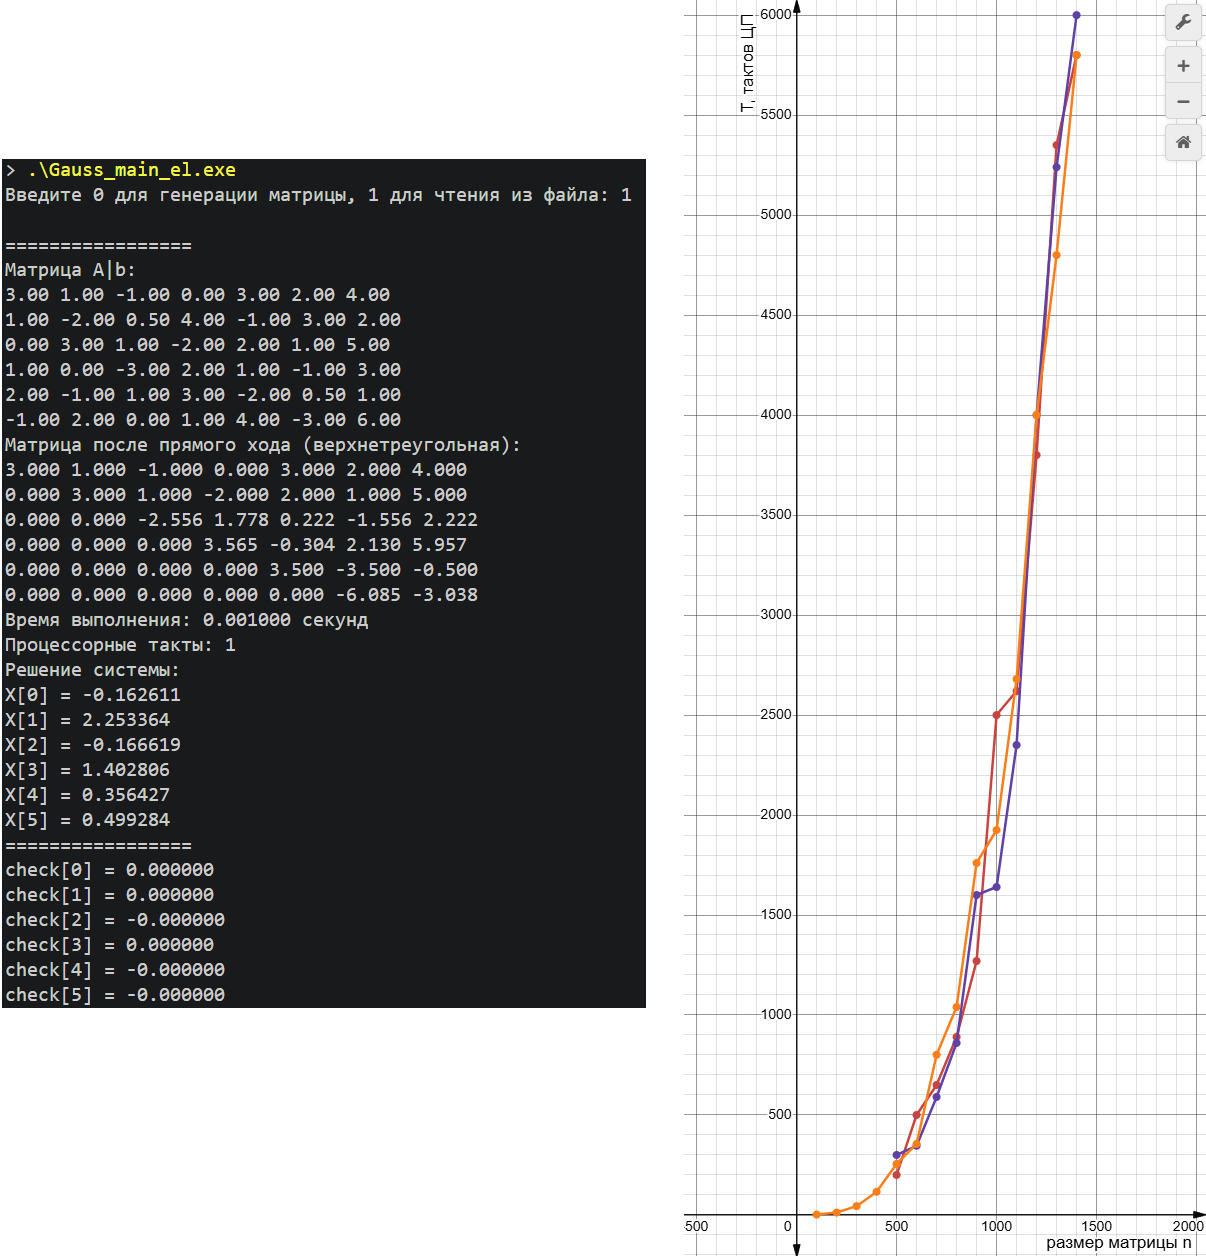
\includegraphics[width=14cm]{График времени выполнения от n.png}
	    %\caption{Зависимость времени выполнения от размера матрицы~$A$}
\end{figure}


Программная реализация на языке C:
\begin{Verbatim}[numbers=left, formatcom=\fontsize{12}{12}\selectfont]
#include <stdio.h>
#include <locale.h>
#include <stdlib.h>
#include <windows.h>
#include <math.h>
#include <time.h>


double* gauss(double **A, int n) {
    // Прямой ход с выбором главного элемента по столбцу
    for (int k = 0; k < n - 1; k++) {
        // 1. Поиск главного элемента в столбце k
        int max_row = k;
        double max_val = fabs(A[k][k]);
        for (int i = k + 1; i < n; i++) {
            if (fabs(A[i][k]) > max_val) {
                max_val = fabs(A[i][k]);
                max_row = i;
            }
        }
        // Проверка на ноль
        if (max_val < 1e-12) {
            printf("Ошибка: столбец %d почти нулевой (главный элемент = %g)\n",
                 k, max_val);
            return NULL;
        }
        // 2. Перестановка строк
        if (max_row != k) {
            double *tmp = A[k];
            A[k] = A[max_row];
            A[max_row] = tmp;
        }
        // 3. Исключение под диагональю
        for (int i = k + 1; i < n; i++) {
            double factor = A[i][k] / A[k][k];
            for (int j = k; j < n + 1; j++) {
                A[i][j] -= factor * A[k][j];
            }
        }
    }

    // Вывод матрицы после прямого хода
    if (n < 10) {
        printf("Матрица после прямого хода (верхнетреугольная):\n");
        for (int i = 0; i < n; i++) {
            for (int j = 0; j < n + 1; j++) {
                printf("%.3f ", A[i][j]);
            }
            printf("\n");
        }
    }

    // Обратный ход с проверкой диагонали
    double *X = (double *)malloc(n * sizeof(double));
    for (int i = n - 1; i >= 0; i--) {
        if (fabs(A[i][i]) < 1e-12) {
            printf("Ошибка: нулевой диагональный элемент на шаге %d\n", i);
            free(X);
            return NULL;
        }
        X[i] = A[i][n];
        for (int j = i + 1; j < n; j++) {
            X[i] -= A[i][j] * X[j];
        }
        X[i] /= A[i][i];
    }
    return X;
}

double* matrix_x_vector_column(double **A, double *X, int n) {
    double *B = (double *)malloc(n * sizeof(double));
    for (int i = 0; i < n; i++) {
        B[i] = 0.0;
        for (int j = 0; j < n; j++) {
            B[i] += A[i][j] * X[j];
        }
    }
    return B;
}

int main() {
    SetConsoleOutputCP(CP_UTF8);
    setlocale(LC_NUMERIC, "C");

    double **A;
    double **A_for_check;
    double *B;
    double *X;
    double *X_target;
    int n;

    int is_use_file = 0; // 0 - не использовать файл, 1 - использовать файл
    printf("Введите 0 для генерации матрицы, 1 для чтения из файла: ");
    scanf("%d", &is_use_file);

    if (is_use_file == 1) { // ИСПОЛЬЗУЕТСЯ ФАЙЛ
        FILE *fp = fopen("matrixA.txt", "r");
        // Чтение размера матрицы
        if (fscanf(fp, "%d", &n) != 1) {
            printf("Ошибка чтения размера матрицы\n");
            fclose(fp);
            return 1;
        }
        // A --- Расширенная матрица коэффициентов (n x (n+1))
        A = (double **)malloc(n * sizeof(double *));
        for (int i = 0; i < n; i++) {
            A[i] = (double *)malloc((n + 1) * sizeof(double));
        }
        // Чтение расширенной матрицы A|b из файла
        for (int i = 0; i < n; i++) {
            for (int j = 0; j < n + 1; j++) {
                if (fscanf(fp, "%lf", &A[i][j]) != 1) {
                    printf("Ошибка чтения элемента матрицы A[%d][%d]\n", 
                        i, j);
                    fclose(fp);
                    return 1;
                }
            }
        }
        //копируем матрицу A для проверки
        A_for_check = (double **)malloc(n * sizeof(double *));
        for (int i = 0; i < n; i++) {
            A_for_check[i] = (double *)malloc((n + 1) * sizeof(double));
            for (int j = 0; j < n + 1; j++) {
                A_for_check[i][j] = A[i][j];
            }
        }
        // Закрытие файла
        fclose(fp);

        // Решение 
        printf("\n=================\nМатрица A|b:\n");
        for (int i = 0; i < n; i++) {
            for (int j = 0; j < n + 1; j++) {
                printf("%.2f ", A[i][j]);
            }
            printf("\n");
        }

        // Вызов функции Гаусса
        clock_t start = clock();
        X = gauss(A, n);
        clock_t end = clock();
        double time_spent = (double)(end - start) / CLOCKS_PER_SEC;
        printf("Время выполнения: %.6f секунд\n", time_spent);
        printf("Процессорные такты: %ld\n", (long)(end - start));

        // Вывод решения
        printf("Решение системы:\n");
        for (int i = 0; i < n; i++) {
            printf("X[%d] = %.6f\n", i, X[i]);
        }
        printf("=================\n");

        double *check = (double *)malloc(n * sizeof(double));
        check = matrix_x_vector_column(A_for_check, X, n);
        for (int i = 0; i < n; i++) {
            check[i] -= A_for_check[i][n]; // вычитаем b[i]
        }
        for (int i = 0; i < n; i++) {
            printf("check[%d] = %.6f\n", i, check[i]);
        }

        // Освобождение памяти
        for (int i = 0; i < n; i++) {
            free(A[i]);
            free(A_for_check[i]);
        }
        free(A);
        free(X);
    }
    else { // НЕ ИСПОЛЬЗУЕТСЯ ФАЙЛ
        int nn = 100;
        //ввод желаемого размера матрицы через консоль
        printf("Введите размер матрицы n: ");
        scanf("%d", &nn);

        for (n = nn; n < 100; n += 100)
        {
            // A --- Расширенная матрица коэффициентов (n x (n+1))
            A = (double **)malloc(n * sizeof(double *));
            for (int i = 0; i < n; i++) {
                A[i] = (double *)malloc((n + 1) * sizeof(double));
            }
            //заполнение матрицы A и B и их объединение в РМК
            X_target = (double *)malloc(n * sizeof(double));

            int a = 1;
            for (int i = 0; i < n; i++) {
                X_target[i] = a;

                for (int j = 0; j < n; j++) {
                    if (i == j)
                        A[i][j] = a; 
                    else
                        A[i][j] = 0.1 * a; 
                }
                a +=1;
            }

            B = matrix_x_vector_column(A, X_target, n);
            
            for (int i = 0; i < n; i++) {
                A[i][n] = B[i];
            }

            if (n < 10) {
                // Решение 
                printf("\n=================\nМатрица A|b:\n");
                for (int i = 0; i < n; i++) {
                    for (int j = 0; j < n + 1; j++) {
                        printf("%.2f ", A[i][j]);
                    }
                    printf("\n");
                }
            }

            // Вызов функции Гаусса
            clock_t start = clock();
            X = gauss(A, n);
            clock_t end = clock();
            double time_spent = (double)(end - start) / CLOCKS_PER_SEC;
            printf("Время выполнения: %.6f секунд\n", time_spent);
            printf("Процессорные такты: %ld\n", (long)(end - start));


            // Вывод решения
            printf("Решение системы:\n");
            if (n < 10)
                for (int i = 0; i < n; i++)
                    printf("X[%d] = %.6f\n", i, X[i]);
            //else for (int i = 0; i < n; i++) printf("%.2f ", X[i]);
            
            printf("=================\n");    

            // Освобождение памяти
            for (int i = 0; i < n; i++) {
                free(A[i]);
            }
            free(A);
            free(X);
            free(B);
            free(X_target);
        }     
    }
    
    return 0;
}
\end{Verbatim}

%=================================================================================
\textbf{2 Метод Ньютона решения системы нелинейных уравнений}

Задача:
\[
\begin{cases}
    f_1(x, y) = x^2 + y^2 - 4 = 0 \\
    f_2(x, y) = x \cdot y - 1 = 0
\end{cases}
\]

Решение:

Построив графики уравнений $f_1(x, y) = 0$ и $f_2(x, y) = 0$, можно увидеть, что они пересекаются в четырех точках, которые являются решениями данной системы нелинейных уравнений. Эти точки можно найти численно с помощью метода Ньютона, используя начальное приближение, выбранное вблизи предполагаемых пересечений.
\begin{figure}[H]
	\centering
	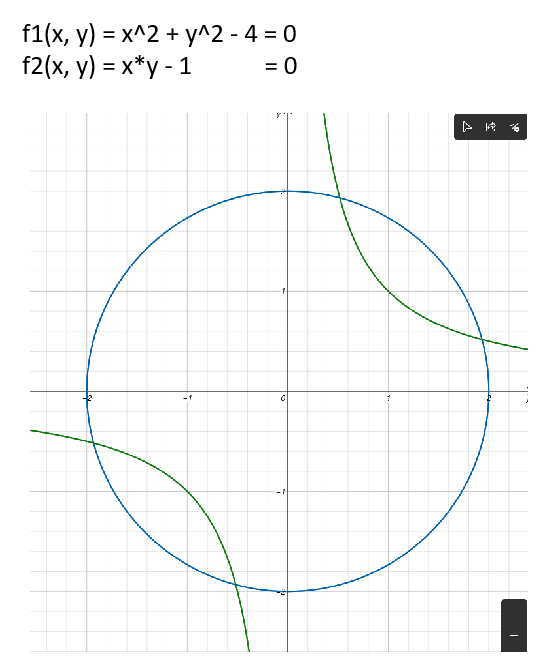
\includegraphics[width=10cm]{For_newton.png}
	    \caption{Графики функций $f_1(x, y) = 0$ и $f_2(x, y) = 0$}
\end{figure}

В результате получаются следующие результаты:
\begin{figure}[H]
	\centering
	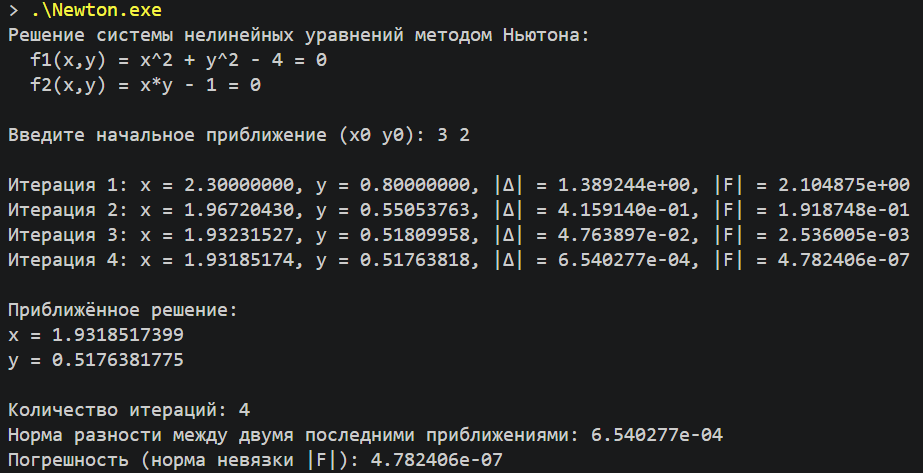
\includegraphics[width=14cm]{Newton_1.png}
	    \caption{Начальное приближение (3, 2)}
\end{figure}
\begin{figure}[H]
	\centering
	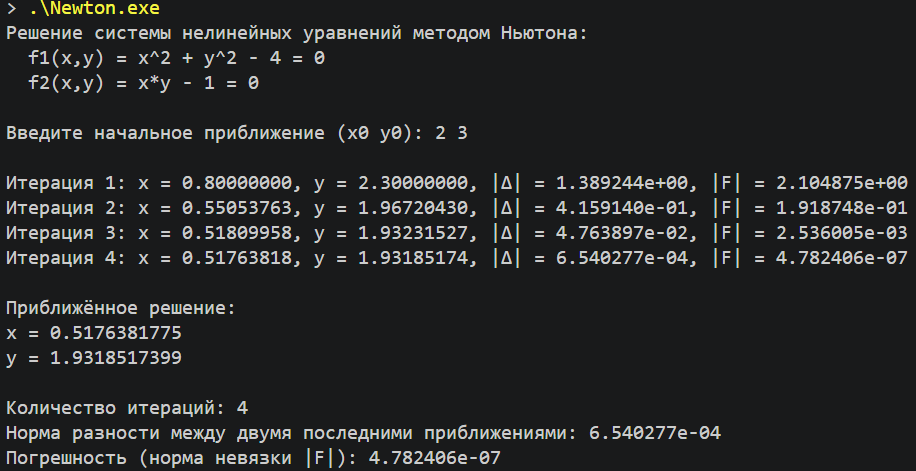
\includegraphics[width=14cm]{Newton_2.png}
	    \caption{Начальное приближение (2, 3)}
\end{figure}
\begin{figure}[H]
	\centering
	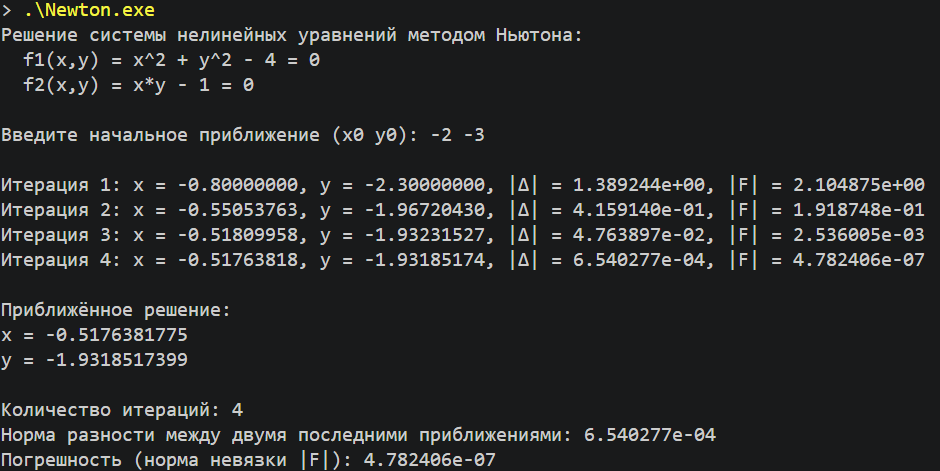
\includegraphics[width=14cm]{Newton_3.png}
	    \caption{Начальное приближение (-2, -3)}
\end{figure}
\begin{figure}[H]
	\centering
	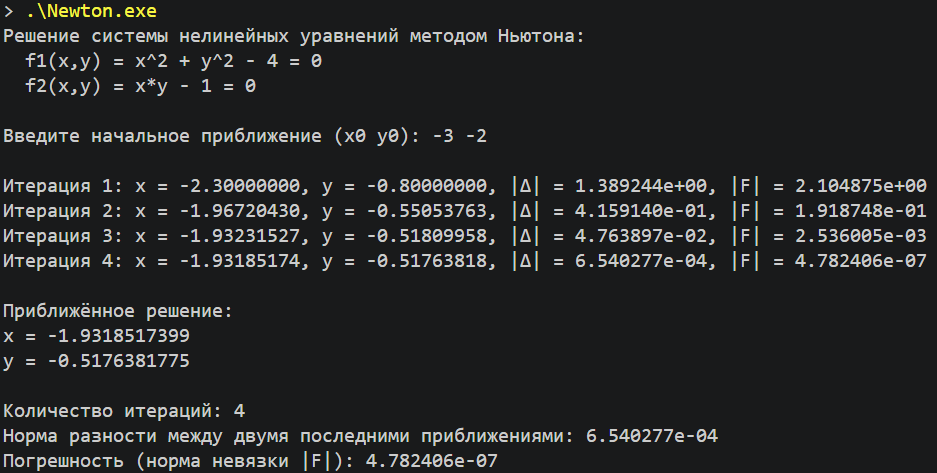
\includegraphics[width=14cm]{Newton_4.png}
	    \caption{Начальное приближение (-3, -2)}
\end{figure}

Программная реализация на языке C:
\begin{Verbatim}[numbers=left, formatcom=\fontsize{12}{12}\selectfont]
#include <stdio.h>
#include <math.h>
#include <locale.h>
#include <stdlib.h>
#include <windows.h>

/* Определение системы нелинейных уравнений:
   f1(x, y) = x^2 + y^2 - 4 = 0
   f2(x, y) = x*y - 1 = 0
*/

double f1(double x, double y) {
    return x * x + y * y - 4.0;
}

double f2(double x, double y) {
    return x * y - 1.0;
}

double df1dx(double x, double y) {
    return 2.0 * x;
}

double df1dy(double x, double y) {
    return 2.0 * y;
}

double df2dx(double x, double y) {
    return y;
}

double df2dy(double x, double y) {
    return x;
}

int main() {
    SetConsoleOutputCP(CP_UTF8);
    setlocale(LC_NUMERIC, "C");

    double x0, y0, eps;
    int max_iter;

    printf("Решение системы нелинейных уравнений методом Ньютона:\n");
    printf("  f1(x,y) = x^2 + y^2 - 4 = 0\n");
    printf("  f2(x,y) = x*y - 1 = 0\n\n");

    eps = 0.0001; // Точность по умолчанию
    max_iter = 100; // Максимальное число итераций по умолчанию

    // Ввод начального приближения
    printf("Введите начальное приближение (x0 y0): ");
    if (scanf("%lf %lf", &x0, &y0) != 2) {
        printf("Ошибка: некорректный ввод начального приближения.\n");
        return 1;
    }
/*
    // Ввод точности
    printf("Введите точность (eps > 0): ");
    if (scanf("%lf", &eps) != 1 || eps <= 0.0) {
        printf("Ошибка: точность должна быть положительным числом.\n");
        return 1;
    }

    // Ввод максимального числа итераций
    printf("Введите максимальное число итераций: ");
    if (scanf("%d", &max_iter) != 1 || max_iter <= 0) {
        printf("Ошибка: max_iter должно быть целым больше нуля.\n");
        return 1;
    }
*/
    printf("\n");

    double x = x0, y = y0;
    int iter;
    // норма разности между двумя последними приближениями
    double norm_delta_last = 0.0;
    // норма невязки в последней точке
    double norm_F_last = 0.0;

    for (iter = 0; iter < max_iter; ++iter) {
        // Вычисление значений функций и матрицы Якоби
        double f1_val = f1(x, y);
        double f2_val = f2(x, y);
        double J11 = df1dx(x, y);
        double J12 = df1dy(x, y);
        double J21 = df2dx(x, y);
        double J22 = df2dy(x, y);

        double det = J11 * J22 - J12 * J21;
        if (fabs(det) < 1e-12) {
            printf("Ошибка: якобиан вырожден (det = %e) на итерации %d\n",
                det, iter);
            break;
        }

        // Решение системы J * delta = -F
        double dx = (-J22 * f1_val + J12 * f2_val) / det;
        double dy = (J21 * f1_val - J11 * f2_val) / det;

        double x_new = x + dx;
        double y_new = y + dy;

        // Норма разности между приближениями
        norm_delta_last = sqrt(dx * dx + dy * dy);

        // Вычисление невязки в новом приближении
        double f1_new = f1(x_new, y_new);
        double f2_new = f2(x_new, y_new);
        norm_F_last = sqrt(f1_new * f1_new + f2_new * f2_new);

        // Печать информации об итерации
        printf("Итерация%2d: x = %.8lf, y = %.8lf, |delta| = %e, |F| = %e\n",
               iter + 1, x_new, y_new, norm_delta_last, norm_F_last);

        // Обновление переменных
        x = x_new;
        y = y_new;

        // Проверка критериев остановки
        if (norm_delta_last < eps || norm_F_last < eps) {
            break;
        }
    }

    // Вывод результатов
    printf("\nПриближённое решение:\n");
    printf("x = %.10lf\n", x);
    printf("y = %.10lf\n", y);
    printf("\nКоличество итераций: %d\n", iter + 1);
    printf("Норма разности между двумя последними приближениями: %e\n",
         norm_delta_last);
    printf("Погрешность (норма невязки |F|): %e\n", norm_F_last);

    if (iter == max_iter && norm_delta_last >= eps && norm_F_last >= eps) {
        printf("\nПредупреждение: достигнуто максимальное число итераций.\n");
    }

    return 0;
}
\end{Verbatim}

%=================================================================================
\textbf{3 Нахождение собственных значений собственых векторов матрицы}
Задача: найти собственные значения и собственные векторы матрицы:
\[
A = \begin{pmatrix}
    5 & 4 & 3 & 2 & 1 \\
    4 & 5 & 4 & 3 & 2 \\
    3 & 4 & 5 & 4 & 3 \\
    2 & 3 & 4 & 5 & 4 \\
    1 & 2 & 3 & 4 & 5
\end{pmatrix}
\]

Программа получает на вход квадратную матрицу, точность и максимальное число итераций. В результате выводятся собственные значения в порядке убывания, соответствующие им собственные векторы, а также проверка невязки $A v - \lambda v$ для каждого найденного собственного вектора.

Вывод программы:
\begin{Verbatim}[formatcom=\fontsize{12}{12}\selectfont]
    Ввод матрицы:
1 - из файла matrix.txt2 - с клавиатуры
Ваш выбор: 1

Введённая матрица:

Исходная матрица:
    5.000000     4.000000     3.000000     2.000000     1.000000 
    4.000000     5.000000     4.000000     3.000000     2.000000 
    3.000000     4.000000     5.000000     4.000000     3.000000 
    2.000000     3.000000     4.000000     5.000000     4.000000 
    1.000000     2.000000     3.000000     4.000000     5.000000 

Введите точность (eps > 0): 0.001
Введите максимальное число итераций: 100

=== РЕЗУЛЬТАТЫ ===
Количество итераций QR-алгоритма: 19

Собственные значения (в порядке убывания):
lambda1 =    17.177798
lambda2 =     5.236068
lambda3 =     1.273771
lambda4 =     0.763930
lambda5 =     0.548434

Собственные векторы (по столбцам):
    0.388330    -0.601501     0.548416    -0.372285     0.219180 
    0.472560    -0.371748    -0.130006     0.603048    -0.507860 
    0.501771     0.000000    -0.604132    -0.002085     0.619069 
    0.472560     0.371748    -0.129686    -0.599948    -0.511599 
    0.388330     0.601501     0.548218     0.371207     0.221491 

=== ПРОВЕРКА A*v - lambda*v ===
Невязка для lambda1 = 2.909515e-09
Невязка для lambda2 = 2.909583e-09
Невязка для lambda3 = 1.357215e-04
Невязка для lambda4 = 6.833356e-04
Невязка для lambda5 = 6.697217e-04
Максимальная невязка: 6.833356e-04
\end{Verbatim}



Программная реализация на языке C:
\begin{Verbatim}[numbers=left, formatcom=\fontsize{12}{12}\selectfont]
#include <stdio.h>
#include <math.h>
#include <stdlib.h>
#include <string.h>
#include <locale.h>
#include <windows.h>

//  ОСНОВНЫЕ ФУНКЦИИ 

double** alloc_matrix(int n) {
    double** A = (double**)malloc(n * sizeof(double*));
    if (A == NULL) return NULL;
    for (int i = 0; i < n; i++) {
        A[i] = (double*)malloc(n * sizeof(double));
        if (A[i] == NULL) {
            for (int j = 0; j < i; j++) free(A[j]);
            free(A);
            return NULL;
        }
    }
    return A;
}

void free_matrix(double** A, int n) {
    if (A == NULL) return;
    for (int i = 0; i < n; i++) free(A[i]);
    free(A);
}

void copy_matrix(double** dest, double** src, int n) {
    for (int i = 0; i < n; i++)
        for (int j = 0; j < n; j++)
            dest[i][j] = src[i][j];
}

void matrix_multiply(double** A, double** B, 
                double** C, int n) {
    double** temp = alloc_matrix(n);
    if (temp == NULL) return;
    for (int i = 0; i < n; i++) {
        for (int j = 0; j < n; j++) {
            temp[i][j] = 0.0;
            for (int k = 0; k < n; k++)
                temp[i][j] += A[i][k] * B[k][j];
        }
    }
    copy_matrix(C, temp, n);
    free_matrix(temp, n);
}

double off_diagonal_norm(double** A, int n) {
    double sum = 0.0;
    for (int i = 0; i < n; i++)
        for (int j = 0; j < n; j++)
            if (i != j) sum += A[i][j] * A[i][j];
    return sqrt(sum);
}

void print_matrix(double** A, int n, const char* title) {
    printf("\n%s:\n", title);
    for (int i = 0; i < n; i++) {
        for (int j = 0; j < n; j++)
            printf("%12.6f ", A[i][j]);
        printf("\n");
    }
}

void print_eigenvalues(double* eigenvals, int n) {
    printf("\nСобственные значения (в порядке убывания):\n");
    for (int i = 0; i < n; i++)
        printf("lambda%d = %12.6f\n", i+1, eigenvals[i]);
}

void print_eigenvectors(double** V, int n) {
    printf("\nСобственные векторы (по столбцам):\n");
    for (int i = 0; i < n; i++) {
        for (int j = 0; j < n; j++)
            printf("%12.6f ", V[i][j]);
        printf("\n");
    }
}

// =============== QR-РАЗЛОЖЕНИЕ (ВРАЩЕНИЯ ГИВЕНСА) 
void qr_decomposition(double** A, double** Q, 
                double** R, int n) {
    for (int i = 0; i < n; i++)
        for (int j = 0; j < n; j++)
            R[i][j] = A[i][j];
    for (int i = 0; i < n; i++)
        for (int j = 0; j < n; j++)
            Q[i][j] = (i == j) ? 1.0 : 0.0;
    
    for (int j = 0; j < n-1; j++) {
        for (int i = n-1; i > j; i--) {
            if (fabs(R[i][j]) > 1e-14) {
                double a = R[i-1][j];
                double b = R[i][j];
                double r = sqrt(a*a + b*b);
                double c = a / r;
                double s = -b / r;
                for (int k = j; k < n; k++) {
                    double temp = c * R[i-1][k] - s * R[i][k];
                    R[i][k] = s * R[i-1][k] + c * R[i][k];
                    R[i-1][k] = temp;
                }
                for (int k = 0; k < n; k++) {
                    double temp = c * Q[k][i-1] - s * Q[k][i];
                    Q[k][i] = s * Q[k][i-1] + c * Q[k][i];
                    Q[k][i-1] = temp;
                }
            }
        }
    }
}

// ============ QR-АЛГОРИТМ 
int qr_algorithm(double** A, double* eigenvalues, 
        double** eigenvectors, int n, double eps, 
        int max_iter, int* iterations_used) 
    {
    double** H = alloc_matrix(n);
    double** Q = alloc_matrix(n);
    double** R = alloc_matrix(n);
    double** newH = alloc_matrix(n);
    double** V = alloc_matrix(n);
    if (!H || !Q || !R || !newH || !V) {
        printf("Ошибка выделения памяти.\n");
        return 0;
    }
    
    copy_matrix(H, A, n);
    for (int i = 0; i < n; i++)
        for (int j = 0; j < n; j++)
            V[i][j] = (i == j) ? 1.0 : 0.0;
    
    int iter = 0;
    double norm = off_diagonal_norm(H, n);
    
    while (norm > eps && iter < max_iter) {
        qr_decomposition(H, Q, R, n);
        matrix_multiply(R, Q, newH, n);
        double** temp = alloc_matrix(n);
        matrix_multiply(V, Q, temp, n);
        copy_matrix(V, temp, n);
        free_matrix(temp, n);
        copy_matrix(H, newH, n);
        norm = off_diagonal_norm(H, n);
        iter++;
    }
    
    *iterations_used = iter;
    
    if (iter >= max_iter) {
        printf("Внимание: достигнуто максимальное число итераций (%d)\n", 
            max_iter);
        printf("Текущая норма внедиагональных элементов: %e\n", norm);
        free_matrix(H, n); free_matrix(Q, n); free_matrix(R, n);
        free_matrix(newH, n); free_matrix(V, n);
        return 0;
    }
    
    for (int i = 0; i < n; i++)
        eigenvalues[i] = H[i][i];
    
    // Сортировка по убыванию
    for (int i = 0; i < n-1; i++) {
        for (int j = i+1; j < n; j++) {
            if (eigenvalues[i] < eigenvalues[j]) {
                double tmp = eigenvalues[i];
                eigenvalues[i] = eigenvalues[j];
                eigenvalues[j] = tmp;
                for (int k = 0; k < n; k++) {
                    double tmp_vec = V[k][i];
                    V[k][i] = V[k][j];
                    V[k][j] = tmp_vec;
                }
            }
        }
    }
    
    // Нормировка векторов
    for (int j = 0; j < n; j++) {
        double norm_vec = 0.0;
        for (int i = 0; i < n; i++)
            norm_vec += V[i][j] * V[i][j];
        norm_vec = sqrt(norm_vec);
        if (norm_vec > 1e-12)
            for (int i = 0; i < n; i++)
                V[i][j] /= norm_vec;
    }
    
    copy_matrix(eigenvectors, V, n);
    
    free_matrix(H, n); free_matrix(Q, n); free_matrix(R, n);
    free_matrix(newH, n); free_matrix(V, n);
    return 1;
}

// ======== ВВОД МАТРИЦЫ 
double** read_matrix_from_file(int* n) {
    const char* fname = "matrix.txt";
    FILE* fp = fopen(fname, "r");
    if (!fp) {
        printf("Не удалось открыть файл %s\n", fname);
        return NULL;
    }
    if (fscanf(fp, "%d", n) != 1 || *n <= 0) {
        printf("Ошибка чтения размера матрицы.\n");
        fclose(fp);
        return NULL;
    }
    double** A = alloc_matrix(*n);
    if (!A) return NULL;
    for (int i = 0; i < *n; i++) {
        for (int j = 0; j < *n; j++) {
            if (fscanf(fp, "%lf", &A[i][j]) != 1) {
                printf("Ошибка чтения элемента матрицы.\n");
                fclose(fp);
                free_matrix(A, *n);
                return NULL;
            }
        }
    }
    fclose(fp);
    return A;
}

double** read_matrix_from_keyboard(int* n) {
    printf("Введите размерность квадратной матрицы n: ");
    scanf("%d", n);
    if (*n <= 0) {
        printf("Размерность должна быть положительной.\n");
        return NULL;
    }
    double** A = alloc_matrix(*n);
    if (!A) return NULL;
    printf("Введите элементы матрицы построчно:\n");
    for (int i = 0; i < *n; i++)
        for (int j = 0; j < *n; j++)
            scanf("%lf", &A[i][j]);
    return A;
}

// ======== ПРОВЕРКА A*v - lambda*v = 0 
void check_residuals(double** A, double* eigenvalues, 
    double** eigenvectors, int n) {
    double max_resid = 0.0;
    printf("\n=== ПРОВЕРКА A*v - lambda*v ===\n");
    for (int j = 0; j < n; j++) {
        double* Av = (double*)malloc(n * sizeof(double));
        double* resid = (double*)malloc(n * sizeof(double));
        // Вычисляем A * v_j
        for (int i = 0; i < n; i++) {
            Av[i] = 0.0;
            for (int k = 0; k < n; k++)
                Av[i] += A[i][k] * eigenvectors[k][j];
            resid[i] = Av[i] - eigenvalues[j] * eigenvectors[i][j];
        }
        double norm_resid = 0.0;
        for (int i = 0; i < n; i++)
            norm_resid += resid[i] * resid[i];
        norm_resid = sqrt(norm_resid);
        free(Av);
        free(resid);
        printf("Невязка для lambda%d = %e\n", j+1, norm_resid);
        if (norm_resid > max_resid) max_resid = norm_resid;
    }
    printf("Максимальная невязка: %e\n", max_resid);
}

//  ОСНОВНАЯ ФУНКЦИЯ 
int main() {
    SetConsoleOutputCP(CP_UTF8);
    setlocale(LC_NUMERIC, "C");
    int n, choice;
    double** A = NULL;
    
    printf("=== QR-АЛГОРИТМ ДЛЯ СИММЕТРИЧНОЙ МАТРИЦЫ ===\n");
    printf("Ввод матрицы:\n1 - из файла matrix.txt");
    printf("2 - с клавиатуры\nВаш выбор: ");
    scanf("%d", &choice);
    
    if (choice == 1) {
        A = read_matrix_from_file(&n);
    } else if (choice == 2) {
        A = read_matrix_from_keyboard(&n);
    } else {
        printf("Неверный выбор.\n");
        return 1;
    }
    
    if (A == NULL) {
        printf("Ошибка при чтении матрицы.\n");
        return 1;
    }
    
    printf("\nВведённая матрица:\n");
    print_matrix(A, n, "Исходная матрица");
    
    // Проверка симметричности (предупреждение)
    int symmetric = 1;
    for (int i = 0; i < n && symmetric; i++)
        for (int j = i+1; j < n; j++)
            if (fabs(A[i][j] - A[j][i]) > 1e-8) 
                { symmetric = 0; break; }
    if (!symmetric) {
        printf("\nПредупреждение: матрица не симметрична!");
        printf(" Алгоритм может работать некорректно.\n");
    }
    
    double eps;
    int max_iter;
    printf("\nВведите точность (eps > 0): ");
    scanf("%lf", &eps);
    printf("Введите максимальное число итераций: ");
    scanf("%d", &max_iter);
    
    double* eigenvalues = (double*)malloc(n * sizeof(double));
    double** eigenvectors = alloc_matrix(n);
    if (eigenvalues == NULL || eigenvectors == NULL) {
        printf("Ошибка выделения памяти.\n");
        free_matrix(A, n);
        return 1;
    }
    
    int iter_used = 0;
    int success = qr_algorithm(A, eigenvalues, eigenvectors, n, eps, max_iter, &iter_used);
    
    if (success) {
        printf("\n=== РЕЗУЛЬТАТЫ ===\n");
        printf("Количество итераций QR-алгоритма: %d\n", iter_used);
        print_eigenvalues(eigenvalues, n);
        print_eigenvectors(eigenvectors, n);
        
        check_residuals(A, eigenvalues, eigenvectors, n);
    } else {
        printf("\nQR-алгоритм не сошёлся за %d итераций.\n", max_iter);
    }
    
    free_matrix(A, n);
    free_matrix(eigenvectors, n);
    free(eigenvalues);
    
    return 0;
}

\end{Verbatim}


%=================================================================================
\end{document}